\section{Flujo de ejecución principal}

La Figura \ref{fig:secuencia-ejecucion} ilustra el flujo de ejecución que se produce cuando el estudiante envía una expresión desde la consola del prototipo, desde la interacción inicial hasta la obtención del resultado en el servidor. El flujo inicia en el componente \texttt{ConsoleOutput}, que delega la acción al orquestador \texttt{PlaygroundLayout}. Este registra la expresión en el historial, inicializa el mecanismo de cancelación y deshabilita nuevas ejecuciones concurrentes. A continuación, invoca el servicio \texttt{racket.ts}, que empaqueta los archivos del editor y la expresión en una petición HTTP POST hacia \texttt{/api/run}. El servidor de aplicación recibe la solicitud, prepara el entorno de ejecución aislado, lanza el proceso Racket, deserializa su salida y devuelve la secuencia de pasos al cliente.

\begin{figure}[H]
    \centering
    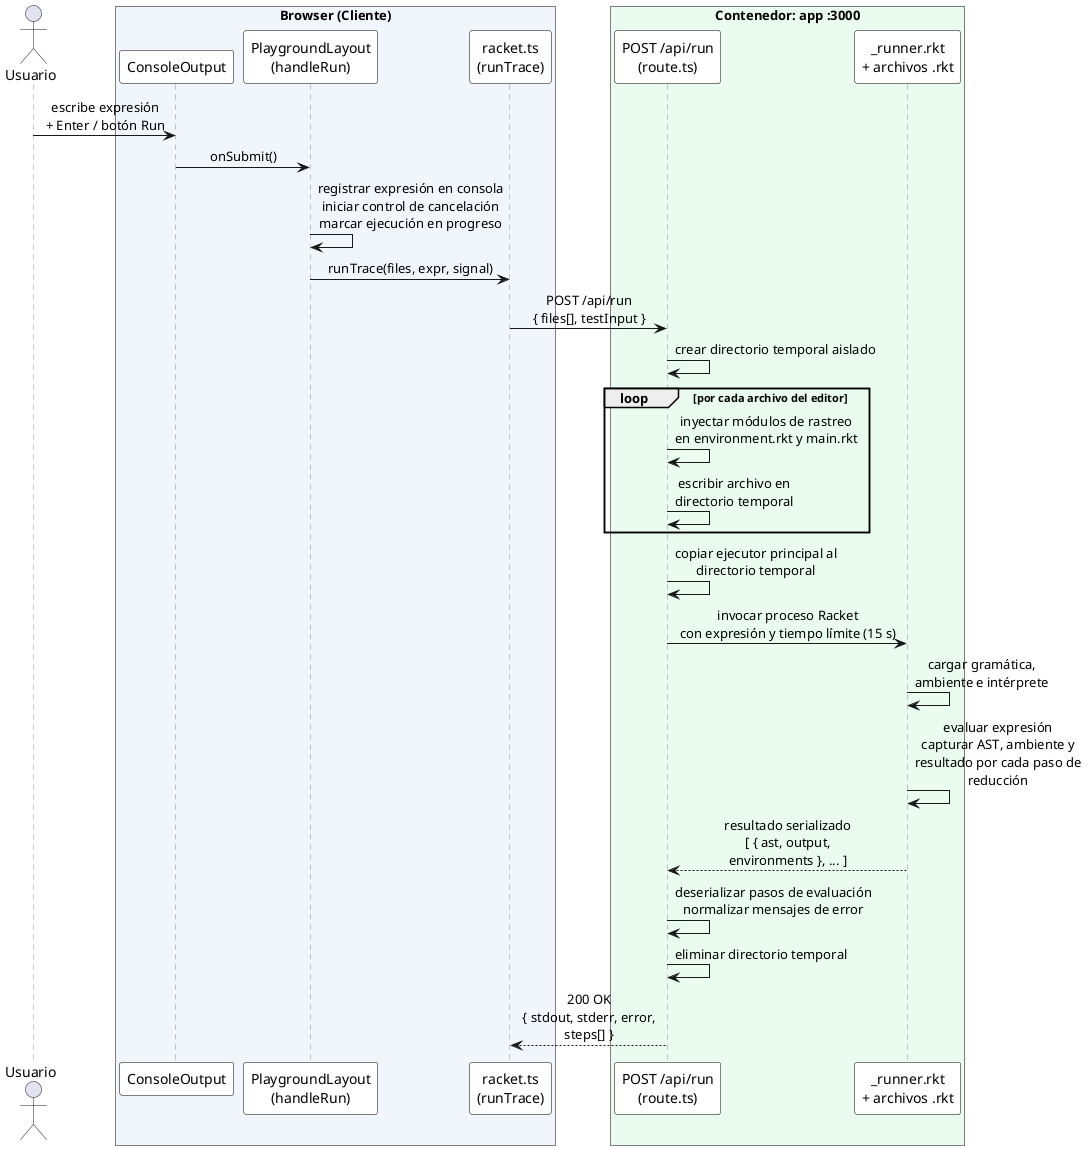
\includegraphics[width=\textwidth,height=0.82\textheight,keepaspectratio]{Capitulo_5/imagenes/secuencia-ejecucion.png}
    \caption{Diagrama de secuencia de la solicitud y evaluación en el servidor del prototipo FLP Viewer}
    \scriptsize \textbf{Fuente:} Elaboración propia
    \label{fig:secuencia-ejecucion}
\end{figure}

\FloatBarrier

Una vez que el cliente recibe la respuesta, \texttt{PlaygroundLayout} distribuye los resultados entre los paneles de visualización según el modo activo, tal como se muestra en la Figura \ref{fig:secuencia-resultado}: en modo normal actualiza el AST, el ambiente y la consola con el estado final, y en modo paso a paso encola los pasos y presenta el primero de forma inmediata, habilitando la navegación manual.

\begin{figure}[H]
    \centering
    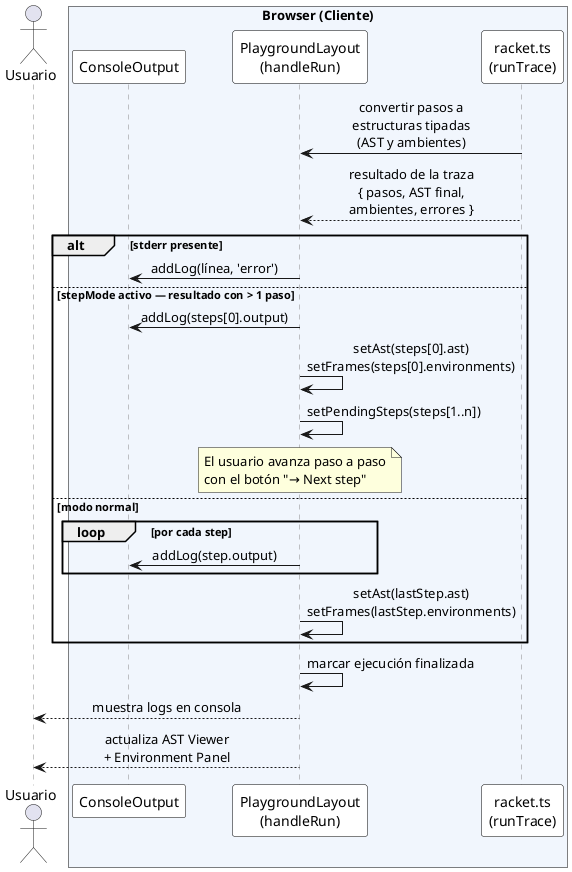
\includegraphics[width=\textwidth,height=0.82\textheight,keepaspectratio]{Capitulo_5/imagenes/secuencia-resultado.png}
    \caption{Diagrama de secuencia de la distribución de resultados en la interfaz del prototipo FLP Viewer}
    \scriptsize \textbf{Fuente:} Elaboración propia
    \label{fig:secuencia-resultado}
\end{figure}

\FloatBarrier
